%%%%%%%%%%%%%%%%%%%%
%%%%%%%%%%%%%%%%%%%%
%%
%% Andrea Tino - 2019
%
%% Programming + Science
%% Cellular Automata
%%
%%%%%%%%%%%%%%%%%%%%
%%%%%%%%%%%%%%%%%%%%


\documentclass[twoside,symmetric,justified]{tufte-book}

\hypersetup{colorlinks}% uncomment this line if you prefer colored hyperlinks (e.g., for onscreen viewing)

%%
% Book metadata
\title{Studying\\populations using\\Cellular Automata}
\author[Andrea Tino]{Andrea Tino}
\publisher{An Open Source Book}

%%
% If they're installed, use Bergamo and Chantilly from www.fontsite.com.
% They're clones of Bembo and Gill Sans, respectively.
%\IfFileExists{bergamo.sty}{\usepackage[osf]{bergamo}}{}% Bembo
%\IfFileExists{chantill.sty}{\usepackage{chantill}}{}% Gill Sans

%\usepackage{microtype}

%%
% Just some sample text
\usepackage{lipsum}

%%
% For nicely typeset tabular material
\usepackage{booktabs}



%%
% TIKZ
\usepackage{tikz}
\usetikzlibrary{plotmarks}
\usetikzlibrary{patterns}
\usetikzlibrary{decorations.markings}
\usetikzlibrary{math}
\usetikzlibrary{matrix}
\usetikzlibrary{arrows,tikzmark,shadows,positioning}

%%
% Algorithms
\usepackage{algorithm}
\usepackage{algpseudocode}

%%
% Misc
\usepackage{xstring}

%%
% Listings
%\usepackage{xcolor}
%\definecolor{light-gray}{gray}{0.90}

\usepackage{listings}
\usepackage{lstlinebgrd}

\lstset{basicstyle=\ttfamily\footnotesize,breaklines=true}

%
% ECMAScript 2015 (ES6) definition
%

\lstdefinelanguage[ECMAScript2015]{JavaScript}[]{JavaScript}{
  morekeywords=[1]{await, async, case, catch, class, const, default, do,
    enum, export, extends, finally, from, implements, import, instanceof,
    let, static, super, switch, throw, try},
  morestring=[b]` % Interpolation strings.
}

%
% JavaScript version 1.1
%

\lstdefinelanguage{JavaScript}{
  morekeywords=[1]{break, continue, delete, else, for, function, if, in,
    new, return, this, typeof, var, void, while, with},
  % Literals, primitive types, and reference types.
  morekeywords=[2]{false, null, true, boolean, number, undefined,
    Array, Boolean, Date, Math, Number, String, Object, window, document},
  % Built-ins.
  morekeywords=[3]{eval, parseInt, parseFloat, escape, unescape},
  sensitive,
  morecomment=[s]{/*}{*/},
  morecomment=[l]//,
  morecomment=[s]{/**}{*/}, % JavaDoc style comments
  morestring=[b]',
  morestring=[b]"
}[keywords, comments, strings]

\lstalias[]{ES6}[ECMAScript2015]{JavaScript}

\lstdefinestyle{JavaScript}{
  language=JavaScript
}
\lstdefinestyle{JavaScript2}{
  language=JavaScript,
  basicstyle=\ttfamily\footnotesize\color{gray}
}
\lstdefinestyle{ES6}{
  language=ES6
}

%%%

\lstnewenvironment{codecss}{}{}

\lstnewenvironment{code}
{
\lstset{style=JavaScript}
}
{
}

\lstnewenvironment{codehtml}
{
\lstset{language=HTML}
}
{
}

\lstnewenvironment{codehtmlh1}[2]
{
\lstset{
        language=HTML,
        linebackgroundcolor={\ifnum\value{lstnumber}<#2\ifnum\value{lstnumber}>#1\color{light-gray}\fi\fi}}
}
{
}

\lstnewenvironment{codeh1}[2]
{
\lstset{
        style=JavaScript,
        linebackgroundcolor={\ifnum\value{lstnumber}<#2\ifnum\value{lstnumber}>#1\color{light-gray}\fi\fi}}
}
{
}

\lstnewenvironment{codeh2}[4]
{
\lstset{
        style=JavaScript,
        linebackgroundcolor={
        \ifnum \value{lstnumber}<#2
          \ifnum\value{lstnumber}>#1
            \color{light-gray}
          \fi
        \else
          \ifnum \value{lstnumber}<#4
            \ifnum \value{lstnumber}>#3
              \color{light-gray}
            \fi
          \fi
        \fi}}
}
{
}

%%
% Colors
\definecolor{folderbg}{RGB}{124,166,198}
\definecolor{folderborder}{RGB}{110,144,169}
\def\FolderSize{4pt}
\tikzset{
  folder/.pic={
    \filldraw[draw=folderborder,top color=folderbg!50,bottom color=folderbg]
      (-1.05*\FolderSize,0.2\FolderSize+5pt) rectangle ++(.75*\FolderSize,-0.2\FolderSize-5pt);  
    \filldraw[draw=folderborder,top color=folderbg!50,bottom color=folderbg]
      (-1.15*\FolderSize,-\FolderSize) rectangle (1.15*\FolderSize,\FolderSize);
  }
}

%%
% For graphics / images
\usepackage{graphicx}
\setkeys{Gin}{width=\linewidth,totalheight=\textheight,keepaspectratio}
\graphicspath{{graphics/}}

% The fancyvrb package lets us customize the formatting of verbatim
% environments.  We use a slightly smaller font.
\usepackage{fancyvrb}
\fvset{fontsize=\normalsize}

%%
% Prints argument within hanging parentheses (i.e., parentheses that take
% up no horizontal space).  Useful in tabular environments.
\newcommand{\hangp}[1]{\makebox[0pt][r]{(}#1\makebox[0pt][l]{)}}

%%
% Prints an asterisk that takes up no horizontal space.
% Useful in tabular environments.
\newcommand{\hangstar}{\makebox[0pt][l]{*}}

%%
% Prints a trailing space in a smart way.
\usepackage{xspace}

%%
% Math
\usepackage{amsmath}  % extended mathematics
\usepackage{amsfonts}  % extended mathematics
\usepackage{amssymb}  % extended mathematics
\usepackage{amsthm}

\newtheorem{theorem}{Theorem}[section]
\newtheorem{corollary}{Corollary}[theorem]
\newtheorem{example}{Example}[theorem]
\newtheorem{problem}{Problem}[theorem]
\newtheorem{proposition}{Proposition}[theorem]
\newtheorem{lemma}[theorem]{Lemma}
\newtheorem{definition}{Definition}[section]

\newcommand{\E}{\mathrm{E}}
\newcommand{\median}{\mathrm{median}}
\newcommand{\Var}{\mathrm{Var}}
\newcommand{\EPE}{\mathrm{EPE}}
\newcommand{\argmin}{\mathop{\mathrm{argmin}}}

%%
% Some shortcuts for Tufte's book titles.  The lowercase commands will
% produce the initials of the book title in italics.  The all-caps commands
% will print out the full title of the book in italics.
\newcommand{\vdqi}{\textit{VDQI}\xspace}
\newcommand{\ei}{\textit{EI}\xspace}
\newcommand{\ve}{\textit{VE}\xspace}
\newcommand{\be}{\textit{BE}\xspace}
\newcommand{\VDQI}{\textit{The Visual Display of Quantitative Information}\xspace}
\newcommand{\EI}{\textit{Envisioning Information}\xspace}
\newcommand{\VE}{\textit{Visual Explanations}\xspace}
\newcommand{\BE}{\textit{Beautiful Evidence}\xspace}

\newcommand{\TL}{Tufte-\LaTeX\xspace}

% Prints the month name (e.g., January) and the year (e.g., 2008)
\newcommand{\monthyear}{%
  \ifcase\month\or January\or February\or March\or April\or May\or June\or
  July\or August\or September\or October\or November\or
  December\fi\space\number\year
}


% Prints an epigraph and speaker in sans serif, all-caps type.
\newcommand{\openepigraph}[2]{%
  %\sffamily\fontsize{14}{16}\selectfont
  \begin{fullwidth}
  \sffamily\large
  \begin{doublespace}
  \noindent\allcaps{#1}\\% epigraph
  \noindent\allcaps{#2}% author
  \end{doublespace}
  \end{fullwidth}
}

% Inserts a blank page
\newcommand{\blankpage}{\newpage\hbox{}\thispagestyle{empty}\newpage}

\usepackage{units}

% Typesets the font size, leading, and measure in the form of 10/12x26 pc.
\newcommand{\measure}[3]{#1/#2$\times$\unit[#3]{pc}}

% Macros for typesetting the documentation
\newcommand{\hlred}[1]{\textcolor{Maroon}{#1}}% prints in red
\newcommand{\hangleft}[1]{\makebox[0pt][r]{#1}}
\newcommand{\hairsp}{\hspace{1pt}}% hair space
\newcommand{\hquad}{\hskip0.5em\relax}% half quad space
\newcommand{\TODO}{\textcolor{red}{\bf TODO!}\xspace}
\newcommand{\ie}{\textit{i.\hairsp{}e.}\xspace}
\newcommand{\eg}{\textit{e.\hairsp{}g.}\xspace}
\newcommand{\na}{\quad--}% used in tables for N/A cells
\providecommand{\XeLaTeX}{X\lower.5ex\hbox{\kern-0.15em\reflectbox{E}}\kern-0.1em\LaTeX}
\newcommand{\tXeLaTeX}{\XeLaTeX\index{XeLaTeX@\protect\XeLaTeX}}
% \index{\texttt{\textbackslash xyz}@\hangleft{\texttt{\textbackslash}}\texttt{xyz}}
\newcommand{\tuftebs}{\symbol{'134}}% a backslash in tt type in OT1/T1
\newcommand{\doccmdnoindex}[2][]{\texttt{\tuftebs#2}}% command name -- adds backslash automatically (and doesn't add cmd to the index)
\newcommand{\doccmddef}[2][]{%
  \hlred{\texttt{\tuftebs#2}}\label{cmd:#2}%
  \ifthenelse{\isempty{#1}}%
    {% add the command to the index
      \index{#2 command@\protect\hangleft{\texttt{\tuftebs}}\texttt{#2}}% command name
    }%
    {% add the command and package to the index
      \index{#2 command@\protect\hangleft{\texttt{\tuftebs}}\texttt{#2} (\texttt{#1} package)}% command name
      \index{#1 package@\texttt{#1} package}\index{packages!#1@\texttt{#1}}% package name
    }%
}% command name -- adds backslash automatically
\newcommand{\doccmd}[2][]{%
  \texttt{\tuftebs#2}%
  \ifthenelse{\isempty{#1}}%
    {% add the command to the index
      \index{#2 command@\protect\hangleft{\texttt{\tuftebs}}\texttt{#2}}% command name
    }%
    {% add the command and package to the index
      \index{#2 command@\protect\hangleft{\texttt{\tuftebs}}\texttt{#2} (\texttt{#1} package)}% command name
      \index{#1 package@\texttt{#1} package}\index{packages!#1@\texttt{#1}}% package name
    }%
}% command name -- adds backslash automatically
\newcommand{\docopt}[1]{\ensuremath{\langle}\textrm{\textit{#1}}\ensuremath{\rangle}}% optional command argument
\newcommand{\docarg}[1]{\textrm{\textit{#1}}}% (required) command argument
\newenvironment{docspec}{\begin{quotation}\ttfamily\parskip0pt\parindent0pt\ignorespaces}{\end{quotation}}% command specification environment
\newcommand{\docenv}[1]{\texttt{#1}\index{#1 environment@\texttt{#1} environment}\index{environments!#1@\texttt{#1}}}% environment name
\newcommand{\docenvdef}[1]{\hlred{\texttt{#1}}\label{env:#1}\index{#1 environment@\texttt{#1} environment}\index{environments!#1@\texttt{#1}}}% environment name
\newcommand{\docpkg}[1]{\texttt{#1}\index{#1 package@\texttt{#1} package}\index{packages!#1@\texttt{#1}}}% package name
\newcommand{\doccls}[1]{\texttt{#1}}% document class name
\newcommand{\docclsopt}[1]{\texttt{#1}\index{#1 class option@\texttt{#1} class option}\index{class options!#1@\texttt{#1}}}% document class option name
\newcommand{\docclsoptdef}[1]{\hlred{\texttt{#1}}\label{clsopt:#1}\index{#1 class option@\texttt{#1} class option}\index{class options!#1@\texttt{#1}}}% document class option name defined
\newcommand{\docmsg}[2]{\bigskip\begin{fullwidth}\noindent\ttfamily#1\end{fullwidth}\medskip\par\noindent#2}
\newcommand{\docfilehook}[2]{\texttt{#1}\index{file hooks!#2}\index{#1@\texttt{#1}}}
\newcommand{\doccounter}[1]{\texttt{#1}\index{#1 counter@\texttt{#1} counter}}

%%%%%%%%%%%%%%%%%%%%%
%%%%%%%%%%%%%%%%%%%%%
%%%%%%%%%%%%%%%%%%%%%

% Generates the index
\usepackage{makeidx}
\makeindex

\begin{document}

% Front matter
\frontmatter


% r.3 full title page
\maketitle


% v.4 copyright page
\newpage
\begin{fullwidth}
~\vfill
\thispagestyle{empty}
\setlength{\parindent}{0pt}
\setlength{\parskip}{\baselineskip}
Copyright \copyright\ \the\year\ \thanklessauthor

\par\smallcaps{Publishing: \thanklesspublisher}

\par\smallcaps{github.com/youth-code-academy/book-programming-science}

\par This work is licensed under the Creative Commons Attribution-NonCommercial-ShareAlike
4.0 International License. To view a copy of this license, 
visit \url{http://creativecommons.org/licenses/by-nc-sa/4.0/} or send a letter to
Creative Commons,
PO Box 1866, Mountain View, CA 94042, USA.\index{license}

\par\textit{First printing, \monthyear}
\end{fullwidth}

% r.5 contents
\tableofcontents

%\listoffigures

%\listoftables

% r.7 dedication
\cleardoublepage
~\vfill
\begin{doublespace}
\noindent\fontsize{18}{22}\selectfont\itshape
\nohyphenation
Dedicated to all the young students I had the privilege to tutor
so far and allowed me to develop this work.
\end{doublespace}
\vfill
\vfill


\cleardoublepage

% Start the main matter (normal chapters)
\mainmatter

%%%%%%%%%%%%%%%%%%%%
%%%%%%%%%%%%%%%%%%%%
%%
%% Andrea Tino - 2019
%% Programming + Science
%% Intro
%%
%%%%%%%%%%%%%%%%%%%%
%%%%%%%%%%%%%%%%%%%%

\section{Introduction - Why and how do we describe populations?}
\label{sec:intro}

A population is a collection of individuals. It does not necessarily need
to be a set of people, it can be animals. It does not even need to include the
same type of elements, populations can be heterogeneous (e.g. a population
of men and women).

Why do we need to describe and analyze these structures? There are many answers
but the most important is certainly: because our societies are organized in populations!
There are populations everywhere: the city where we live, the building where we reside,
the means of transport we use everyday, the roads we fill with our cars, bycicles and
scooters and so forth. We describe things because we want to extract information, knowledge
that we can use later to achieve some level of control. A practical example is traffic
lights: a crossroad is a limited space where a population of cars happens to spend a
relatively short amount of time.
If we gain more information about the population of cars entering and exiting an
intersection, we can later create an algorithm to rework the time durations of green vs.
red signals at each joining road to maximize the 
throughput\footnote{The amount of something in unit of time: $\eta = \frac{N}{T}$. 
Throughput is most often a measure of speed.}.

Urban networks is not the only case scenario where population study comes handy. Other
examples include Biology and Virology: how does an infection propagate over a closed
population of individuals? Kermack \& McKendrick \cite{kermack-mckendrick}
gave an answer to that question by formulating what is known, today, as the \textit{SIR} model
\cite{kermack-mckendrick-sir}, widely used today everytime an epidemic occurs in the world. The
model was recently used in the outbreak of the T-virus and Ebola virus in Africa in order to
come up with good and effective containment strategies to avoid worldwide spread.

One final example of the application of population study concerns relationships among two or more
populations. Lotka \& Volterra \cite{lotka-volterra} created a model for describing how
the sub-populations of predators and preys interact together. This model was recently used, for example,
to try to find a solution to the problem of extinction in the population of Zebras in Kongo.\\

Now that you are, hopefully, convinced of the importance of studying populations, let's answer the
second question: how do we analyze populations?

There are many approaches that have been put in practice and published so far. A generic approach cannot
really be considered because the strategies vary case by case, depending on the type of population
and what exactly is the the focus of the research. In the afore-mentioned examples, both
Kermack-McKendrick and Lotka-Volterra studies employ
compartmentalized\footnote{A population is seen as a compartment: a basin. In this description, each
individual does not really count, the measure which is considered is the total amount of individuals
in the group and how this number changes over time.}
models to describe,
respectively, the population of people being infected, and the populations of preys and predators.
However other models have been used to tackle the same problem. In the case of Kermack-McKendrick,
for example, contact between individuals of a population is modeled using graphs, this helps
having a better description of how a virus can spread.

So, as you can see, different mathematical models can be used to solve the same problem. 
It is important to highlight how every model has a different descriptive power that allows us to
be in control of different aspects of the environment we want to study. In this chapter,
we focus on one category of these called: \textit{Cellular Automata} (CA).

\subsection{What are Cellular Automata?}
A CA is a mathematical model built on the following base concepts:

\begin{itemize}
\item \textbf{Population:} A set of individuals is at the center of the description.
\item \textbf{Connecctivity:} A CA is able to define relationships between different individuals in
the population These connections will affect the behavior of the whole population.
\item \textbf{Structure:} The individuals os the population are arranged in a regular geometrical structure
which also affects the connections among individuals.
\item \textbf{Collective vs individual behavior:} A CA is capable of visualizing the state of each single
member as well as the collective state of the whole population.
\end{itemize}

Because of these fundamental characteristics, CA play a key role in population study today. Let's have
a look at how a Cellular Automaton is defined and works, starting with:

\begin{definition}[Alphabet]
\label{def:alpha}
An \textit{alphabet} $\mathcal{A}$ is a set of symbols that is used to describe
the \textit{state} of every individual of a population.
\end{definition}

What do we mean by \textit{state}? 

\begin{definition}[State]
\label{def:state}
Each single individual of the population can be described with a fixed set of properties that will represent
it during time. At each instant, the values of these properties will determine the state of the individual.
\end{definition}

Let's make a few examples.

\begin{example}[State in a SIR model]
\label{ex:statesir}
We mentioned the SIR model before. Though it does not employ CA, the concept of state is still applicable.
This model is used to describe the spread of a virus in a population.
The state, is prepresented by the individual's condition in relation to the virus; at each time, an individual can either be: \textit{Susceptible} (it has not yet been infected by the virus),
\textit{Infected} (it has been infected by the virus and is capable of passing it to others) or
\textit{Removed} (it has recovered from the virus, or it has been killed by it. Either way,
it cannot pass the virus on anymore).
\end{example}

\begin{example}[State in grid of LEDs]
\label{ex:stateled}
Let's consider a grid of LED lights (simple light bulbs are ok too, but LEDs
consume less energy so they are more eco-friendly). At every instant, each light can either be on or off,
which are all the possible states in this context.
\end{example}

So, given definitions \ref{def:alpha} and \ref{def:state}, every member of a population has a state
$a \in \mathcal{A}$ which is an element of the alphabet; this means that the set of states
is, basically, the alphabet.
In example \ref{ex:statesir}, the set of states is $\mathcal{A} = \{ S, I, R \}$. In example
\ref{ex:stateled}, the alphabet is $\mathcal{A} = \{ 0, 1 \}$ ($0$ is off, and $1$ is on).

A CA generates connections between members of the population by arranging them in a very specific
geometrical structure.

\begin{definition}[Cell]
\label{def:cell}
In a CA, a \textit{cell} is a member of the population. The set of all cells is indicated by $E$.
\end{definition}

So from now on, every time we refer to individuals in a population, we can use the term \textit{cell}.
As we already mentioned, every cell has a state. We indicate the state of a cell
$y_{i,j}$ by writing: $y_{i,j} = a$ where $a \in \mathcal{A}$.\\

All the cells in a CA form a shape, this shape will then affect how the cells can be connected together.
We will not talk about the formal model of cell arrangement in CA because it requires many concepts from
Algebra and Set Theory. For our analysis, we can simply consider one very common arrangement of cells:
\textit{$\mathbb{Z}$/$n\mathbb{Z}$ Cellular Automata}\footnote{Also known as: 
\textit{Cellular Automata over rings of integers modulo $n$}.}. It sounds complicated but it actually
is not because they simply are CA where the cells form a grid. In this arrangement, every cell 
(except for those on the border) is surrounded by other 8 cells.
To simplify the notation, to indicate a cell, we can use the following writing: $y_{i,j}$ (with
$i,j \in \mathbb{N}$) to refer to the $i$-th row and $j$-th column in the grid from the top left corner.

\begin{example}[States in grid of LEDs]
\label{ex:stateled2}
With reference to example \ref{ex:stateled}, we can consider a 1x3 grid of lights (a simple line).
At a given time, we can have the situation where the first and the last lights only are on, and
the middle light is off. We can indicate this by writing: $y_{1,1}=1$, $y_{1,2}=0$ and $y_{1,3}=1$. 
\end{example}

\begin{definition}[Neighborhood]
\label{def:neigh}
Every cell $y_{i,j} \in E$ in a CA has a \textit{neighborhood} which is indicated by: 
$B_r\left( y_{i,j} \right)$. It is a set containing all the cells that are connected to
$y_{i,j}$ and have distance $r \in \mathbb{N}$ from it. Note that the neighborhood of a cell does
not contain the cell itself: $y_{i,j} \not\in B_r\left( y_{i,j} \right)$.
\end{definition}

\begin{definition}[Moore neighborhood]
\label{def:neighmoore}
Given a cell $y_{i,j} \in E$ in a CA, its Moore neighborhood $B^\text{M}_r\left( y_{i,j} \right)$
includes all the cells surrounding
$y_{i,j}$.
\end{definition}

\begin{definition}[Von Neumann neighborhood]
\label{def:neighmoore}
Given a cell $y_{i,j} \in E$ in a CA, its Von Neumann neighborhood $B^\text{VN}_r\left( y_{i,j} \right)$
includes only the cells that are
directly adjacent to $y_{i,j}$.
\end{definition}

% For figures use
%
\begin{figure}[b]
\sidecaption
% tikz diagram
%
% Tikz Diagram
%

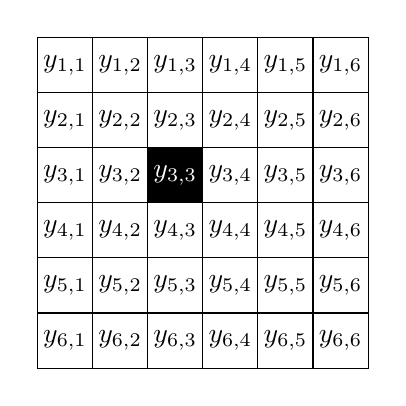
\begin{tikzpicture}

\tikzmath{
	\S = 0.7cm;
}

\tikzset{square matrix/.style={
    matrix of nodes,
    column sep=-\pgflinewidth, row sep=-\pgflinewidth,
    nodes={draw,
      minimum height=#1,
      anchor=center,
      text width=#1,
      align=center,
      inner sep=0pt
    },
  },
  square matrix/.default=\S
}

\matrix[square matrix]
{
$y_{1,1}$ & $y_{1,2}$ & $y_{1,3}$ & $y_{1,4}$ & $y_{1,5}$ & $y_{1,6}$ \\
$y_{2,1}$ & $y_{2,2}$ & $y_{2,3}$ & $y_{2,4}$ & $y_{2,5}$ & $y_{2,6}$ \\
$y_{3,1}$ & $y_{3,2}$ &|[fill=black,text=white]| $y_{3,3}$ & $y_{3,4}$ & $y_{3,5}$ & $y_{3,6}$ \\
$y_{4,1}$ & $y_{4,2}$ & $y_{4,3}$ & $y_{4,4}$ & $y_{4,5}$ & $y_{4,6}$ \\
$y_{5,1}$ & $y_{5,2}$ & $y_{5,3}$ & $y_{5,4}$ & $y_{5,5}$ & $y_{5,6}$ \\
$y_{6,1}$ & $y_{6,2}$ & $y_{6,3}$ & $y_{6,4}$ & $y_{6,5}$ & $y_{6,6}$ \\
};

\end{tikzpicture}

%
% If not, use
%\picplace{5cm}{2cm} % Give the correct figure height and width in cm
%
\caption{If the width of the figure is less than 7.8 cm use the \texttt{sidecapion} command to flush the caption on the left side of the page. If the figure is positioned at the top of the page, align the sidecaption with the top of the figure -- to achieve this you simply need to use the optional argument \texttt{[t]} with the \texttt{sidecaption} command}
\label{fig:exampleca}
\end{figure}
%

\begin{example}[CA with Moore neighborhood and binary states]
\label{ex:simpleca}
Figure \ref{fig:exampleca} shows a simple square 6x6 CA
where the alphabet is $\mathcal{A}=\{ 0, 1 \}$ and the
cells are: $E = \left\{ y_{i,j} : i,j = 1 \dots 6 \right\}$. The neighborhood of cell $y_{3,3}$
is shown, as it is possible to see, it is a Moore neighborhood because all surrounding cells are
included.
\end{example}

\begin{example}[Von Neumann neighborhood]
\label{ex:vnneigh}
With reference to example \ref{ex:simpleca}, we can also see the Van Neumann neighborhood of
cell $y_{4,4}$. In this case, not how only the North, East, South and West surrounding cells
are included.
\end{example}

\begin{important}{Important}
We are going to use always the Moore neighborhood for our analysis, also we will only consider
unit-radius neighborhoods ($r=1$). So, from now on we will always implicitely consider:
$B\left( y_{i,j} \right) = B^\text{M}_1\left( y_{i,j} \right)$.
\end{important}

The last information we need to add about CA, before we can start playing with them, is time.
CA are dynamic objects, they change in time. Before we talk about how they change, we need to
understand how time is modeled in a CA. In mathematical jargon, we say that time is 
\textit{discrete} or, in engineering terms, \textit{slotted}. Normally time is always seen as a
\textit{continuous} entity: a real number: $t \in \mathbb{R}$; thanks to this extreme level of
granularity, we can identify a time instant using a decimal number with a level of precision as high
as we wish (number of decimal digits).
A date and a time can always be converted into a single real number,
the 5\textsuperscript{th} of June 2019 15:55:35 is a date and time that can be converted into seconds
(after Christ's birth), in this case that number would (approximately) be:
\begin{align*}
2019 y + 6 m + 5 d + 15 h + 55 m + 35 s &=\\
2019 \cdot 12 m + 6 \cdot 30 d + 5 \cdot 24 h + 15 \cdot 60 m + 55 \cdot 60 s + 35 s &=\\
2019 \cdot 12 \cdot 30 d + 6 \cdot 30 \cdot 24 h + 5 \cdot 24 \cdot 60 m +
    15 \cdot 60 \cdot 60 s + 3300 s + 35 s &=\\
2019 \cdot 12 \cdot 30 \cdot 24 h + 6 \cdot 30 \cdot 24 \cdot 60 m
    + 5 \cdot 24 \cdot 60 \cdot 60 s +
    54000 s + 3335 s &=\\
2019 \cdot 12 \cdot 30 \cdot 24 \cdot 60 m + 6 \cdot 30 \cdot 24 \cdot 60 \cdot 60 s
    + 432000 s + 57335 s &=\\
2019 \cdot 12 \cdot 30 \cdot 24 \cdot 60 \cdot 60 s + 15552000 s + 489335 s &=\\
62798976000 s + 16041335 s &= 62815017335 s
\end{align*}
Of course, that is not the exact number, as we have simplified things by considering one month always
to be 30 days. But you get the idea. That final number represents
the exact moment when I blew my candels during my birthday this year. And if I had had a stopwatch, I could
even count the milliseconds and add them as a decimal part. This (continuous) vision of time is ideal
when we want to be able to pinpoint an exact instant.

However we don't always need that much precision, sometimes we just want to count events. For example,
we want to count the number of participants at the opening ceremony of every Olympic Game so far.
Those are single events in time, it does not matter to have the precise date and time, we could
just use a natural number to indicate which edition of the Games we are considering. In this example,
we chose to describe time as a \textit{discrete} variable, which means that $t \in \mathbb{N}$.\\

So, now that we have understood time, we can move forward and talk about \textit{evolution}.
CA are very dynamic systems, but so far we have only seen a bunch of cells, each one with a state and
that's it. Well the whole idea is that the CA will change (evolve) in time. This evolution is
represented by a change in the state of every single cell. But how does it happen?

In a CA, time is discrete. The type of events that will make time change depends on the specific model,
hence, at the moment, we just consider time as a meaningless natural number $t \in \mathbb{N}$
that indexes the $t$-th cycle of evolution; once we get to work on a specific model, each cycle will
actually represent something.
At every cycle $t$,
the state of every cell might be different or the same from cycle $t-1$, and this mutation will make
the CA change \textit{configuration} every time.

\begin{definition}[CA configuration]
The \textit{configuration} of a CA at time $t \in \mathbb{N}$, is the set of states of all cells
in the CA at that time: $x_t = \left\{ y^{(t)}_{i,j} \in E \right\}$, where
$y^{(t)}_{i,j}$ represents the state of cell $y_{i,j}$ at time $t$.
\end{definition}

And here comes the final question: how does the state of a cell change? This is where its
neighborhood comes into play.
What is the purpose of a cell's neighborhood? As we mentioned before in definition \ref{def:neigh},
the neighborhood of $y_{i,j}$ contains all the cells $y_{h,k}$ to which $y_{i,j}$ is connected to.
In a CA, the connections are extremely important because the state of one cell will change depending
on the state of every neighbor cell. That's it: the future state of a cell is (also, not only)
determined by the state of its neighbor cells.

\begin{proposition}[Cell state change]
\label{prop:statechange}
In a CA, the state of a cell $y_{i,j} \in E$ in the next cycle $t+1$ depends on 3 factors:
\begin{enumerate}
\item The current cell's state: $y^{(t)}_{i,j}$.
\item The current state of all its neighbor cells: $y^{(t)}_{h,k} \in B\left( y_{i,j} \right)$.
\item Other conditions, specific to the model.
\end{enumerate}
\end{proposition}

When we take proposition \ref{prop:statechange} and write it in mathematical terms, we
get the following:

\begin{definition}[State transition function]
\label{def:statetransf}
Given a CA, we introduce the \textit{cell state transition function}:
\begin{equation}
y^{(t+1)}_{i,j} = f \left[ y^{(t)}_{i,j}, 
    \left\{ y^{(t)}_{h,k} : y_{h,k} \in B\left( y_{i,j} \right) \right\}, \cdot \right]
\end{equation}
Function $f$ defines how the three factors in proposition \ref{prop:statechange}
are used to compute the next state of a cell. $f$ is different in every model.
\end{definition}

Enough with theory, let's make an example.

\begin{example}[Evolution of the LED grid CA]
\label{ex:stateled3}
Recalling example \ref{ex:stateled2}, let's see how we can define a transition function for our
1x3 LED grid to show how this CA can evolve in time. In order to design $f$, we need to define
a neighborhood for each cell. In this simple example, we set every cell to have only one neighbor:
the cell to its right. This means that: $B\left( y_{1,1} \right) = \left\{ y_{1,2} \right\}$,
$B\left( y_{1,2} \right) = \left\{ y_{1,3} \right\}$ and 
$B\left( y_{1,3} \right) = \left\{ y_{1,1} \right\}$ (as you can see, the last cell's
neighbor is the first cell).
Recall that $f$ needs the current cell
and all its neighbors to work, so its input will always be two cells.
In this example, we decide to design $f$ as follows:
\begin{equation*}
f \left( y, y^\prime \right) =
  \begin{cases}
    0       & \quad y = 0 \wedge y^\prime = 0\\
    1       & \quad y = 0 \wedge y^\prime = 1\\
    1       & \quad y = 1 \wedge y^\prime = 1\\
    0       & \quad y = 1 \wedge y^\prime = 0
  \end{cases}
\end{equation*}
Where, $y \in E$ is the current cell and $y^\prime \in E$ its neighbor.
Function $f$ will set the next state in every cell at every cycle $t \in \mathbb{N}$. If we have a look
at its definition, we see that it works in a simple way: the current cell will assume, in $t+1$, the state
of its neighbor at cycle $t$. In fact, the above definition can be simplified as:
\begin{equation*}
f \left( y, y^\prime \right) = y^\prime
\end{equation*}
Let's now have a look at how the CA changes according to $f$ so defined.
We need to set an initial configuration for the CA at $t=0$; this cycle is special as it is the
\textit{initial cycle}. Let's indicate with 
$x_t = \left[ y^{(t)}_{1,1}, y^{(t)}_{1,2}, y^{(t)}_{1,3} \right]$ the configuration of the CA
at cycle $t$. If we start from this initial condition:
$x_0 = (0,0,0)$, how will the CA evolve? The next state of the first cell, is the state of the second
cell, which is $0$. So is the next state of the second cell and the third: $x_1 = (0,0,0)$. If we try
to compute the configuration for the next cycle, we will get the same result. This CA, when given
such an initial condition, will not evolve at all, it will remain the same.

Let's try another initial condition: $x_0 = (0,1,0)$. In this scenario, the middle LED is on.
If we compute the next configuration, we get: $x_1 = (1,0,0)$. If we move on to the next cycle:
$x_2 = (0,0,1)$. And, the next cycle: $x_3 = (0,1,0)$, the CA goes back to its initial condition
to start over again. In this specific scenario, we would see the LEDs creating a cycling linear pattern.
\end{example}

\begin{example}[Another flavor of the LED grid CA]
\label{ex:stateled4}
We keep the same setting of example \ref{ex:stateled3} and change one thing: the transition function
as follows:
\begin{equation*}
f \left( y, y^\prime \right) =
  \begin{cases}
    0       & \quad y = 0 \wedge y^\prime = 0\\
    1       & \quad \text{otherwise}
  \end{cases}
\end{equation*}
Now the CA will work differently from the one in the previous example. Here, in fact, the rule is
that a LED will be stay off only if it is currently off and so is its neighbor. With this
new $f$, let's see what happens when we use the same initial conditions in example \ref{ex:stateled3}.

It is quite trivial to see that the null initial state $x_0 = (0,0,0)$ will cause the CA to behave
like the previous one: no evolution, all LEDs will always remain off.

So let's try the other initial condition: $x_0 = (0,1,0)$. In the first cycle: $x_1 = (1,1,0)$.
In the second cycle, we have: $x_2 = (1,1,1)$. From now on, the CA will remain the same, keeping
configuration $x_t = x_2, \forall t > 2$. So, in this particular CA, when we start with one LED on,
all LEDs will eventually become on.
\end{example}

\begin{problem}
Check that, in example \ref{ex:stateled4}, all initial configurations different from $(0,0,0)$ will
make the CA evolve towards state $(1,1,1)$.
\end{problem}

Thanks to examples \ref{ex:stateled3} and \ref{ex:stateled4}, we have learnt a few important
aspects of CA which are worth mentioning.

\begin{theorem}[CA evolution and initial conditions]
\label{theo:evinitcond}
Given a CA, its evolution depends on the initial condition $x_0$.
\begin{proof}
In both examples \ref{ex:stateled3} and \ref{ex:stateled4}, we could see how the same CA behaved
differently when started from two different initial conditions.
\end{proof}
\end{theorem}

In the example we saw before, we could see how a CA starts from an initial condition 
to reach, possibly, some sort of destination:

\begin{definition}[Final configuration]
\label{def:finalconf}
Given an initial condition/configuration $x_0$, 
it is possible that a CA evolves into a configuration
$x^\ast$ which, once taken, will never be abandoned. If such a configuration exists, we call it
a \textit{final configuration}. When this happens, we write:
$x_0 \overset{f}{\rightarrow} x^\ast$.
We also say that the CA \textit{converges} to $x^\ast$ from $x_0$.
\end{definition}

In example \ref{ex:stateled4}, we could see that any initial configuration with at least one
LED on will lead to all LEDs on. In the specific case, we saw that:
$(0,1,0) \overset{f}{\rightarrow} (1,1,1)$.

\begin{proposition}[Static condition]
When an initial condition $x_0$ causes a CA not to change (not to evolve), we say that
$x_0$ is a \textit{static configuration}.
\end{proposition}

In example \ref{ex:stateled3}, we saw that $(0,0,0)$ is a static configuration.

\begin{proposition}[Recurrent condition]
When an initial condition $x_0$ causes a CA to change different configurations and, after
$T \in \mathbb{N}$ cycles, take that same initial condition and repeat the cycle, we say
that $x_0$ is a \textit{cyclic (or recurrent) configuration of period $T$}.
\end{proposition}

In example \ref{ex:stateled3}, we saw that $(0,1,0)$ is a cyclic configuration of period 3.

\begin{problem}
Prove that, in example \ref{ex:stateled3}, initial condition $(1,0,1)$ is a cyclic configuration
and calculate its period.
\end{problem}

We now know the essentials about CA, we can start creating some interesting models.





%%
% The back matter contains appendices, bibliographies, indices, glossaries, etc.

\backmatter

\bibliography{bibliography}
\bibliographystyle{plainnat}

%%
\printindex

\end{document}

